
\begin{figure}[H]
	\centering
	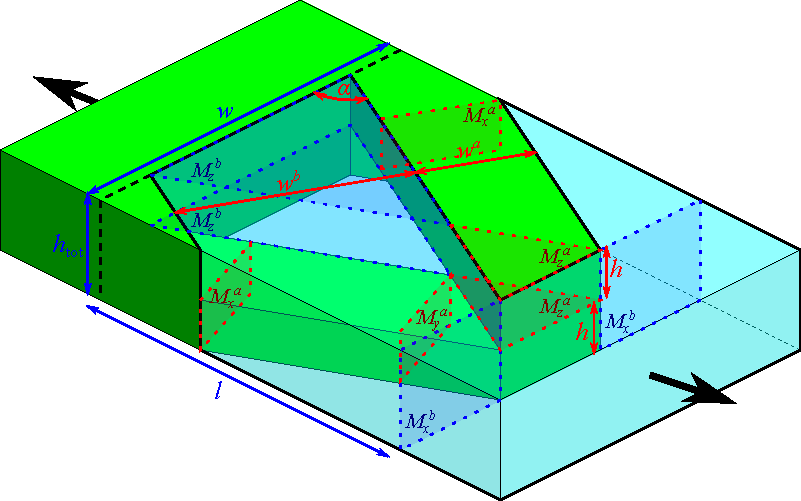
\includegraphics[width=\columnwidth]{sources/method/diagonal_model_v3.pdf}
	\caption{
		One diagonal unit cell connecting material $a$ (left) to material $b$ (right).
		Failure can happen along both the fingers ($M_x$), twice along one finger ($M_y$) or at the interface between the two fingers ($M_z$) for either material.}
	\label{fig:diagonal_model}
\end{figure}


\section{Diagonal Design}

Another option is to place the fingers under an angle as shown in \cref{fig:diagonal_model}.
There are four variables: the finger width of both materials: $w_a$ and $w_b$, the length $L$ and the layer thickness $h$. 
If all four variables are scaled, then the objective function and the constrained functions scale with the same factor. 
Therefore, the layer thickness $h$ will be fixed to $h = \hmin$ and only the variables $w_a$, $w_b$ and $L$ will be optimized.

\subsection{Problem Formulation}
This section shows the deriviation of the problem formulation.

\subsubsection{Geometry Relations}
From \cref{fig:diagonal_model}, the geometry relations \cref{eq:tan,eq:cos,eq:sin} can be derived, which are used for further analysis of the stresses.

\begin{equation}
	\label{eq:tan}
	\tan \alpha = \frac{2L}{w_a + w_b}
\end{equation}

\begin{equation}
	\label{eq:cos}
	\cos \alpha = \frac{w_a + w_b}{\sqrt{ \left( w_a + w_b \right) ^2 + 4L ^2 }}
\end{equation}

\begin{equation}
	\label{eq:sin}
	\sin \alpha = \frac{2L}{\sqrt{ \left( w_a + w_b \right) ^2 + 4L ^2 }}
\end{equation}


\subsubsection{Tension Failure M\textsubscript{x}}\label{ssec:tensfail}
For the tension failure, we consider the smallest cross sectional area of one finger, which is equal to $w_m h \sin \alpha$ . 
The tensile force perpendicular to this area is equal to $\frac{F}{\sin \alpha}$, where $F$ is the force per finger. 
%which was divided by 2 because every finger takes up half of the load. ? - adjust later maybe
Working out $\frac{F}{A} \le \sigma$ resulted in \cref{eq:tensfail}


\begin{equation}
	\label{eq:tensfail}
	\frac{F}{w_m  h} \le \sigma_{max}
\end{equation}


\subsubsection{Shear Failure M\textsubscript{x}}
The same cross sectional area was taken as in \cref{ssec:tensfail}, but now the force that is aligned with this cross section $F \cos \alpha$ is used to evaluate the shear forces. 
The maximum shear stress for a rectangular cross sectional area is equal to $\frac{3V}{2A}$. 
In this way, we derived \cref{eq:shearfailtemp}

\begin{equation}
	\label{eq:shearfailtemp}
	\frac{3F \cos \alpha}{w_m h \sin \alpha} = \frac{3F }{w_m h \tan \alpha} \le \tau_m
\end{equation}

We plugged in \cref{eq:tan} what resulted in \cref{eq:shearmx}.
\begin{equation}
	\label{eq:shearmx}
	\frac{ 3 F \left(w_a + w_b \right) }{ 4  w_m h L} \le \tau_m	
\end{equation}

\subsubsection{Shear Failure M\textsubscript{z}}
For a triangular cross section, the maximum shear stress is equal to $\frac{3F}{bh}$, where $b$ and $h$ are the base and the height of the triangle. 
The width and height of the rectangular area that is loaded in shear are equal to $w_m$ and $\frac{w_m \tan \alpha}{2} $ respectively. 
Combining with \cref{eq:tan} gave \cref{eq:shearMz}.

\begin{equation}
	\label{eq:shearMz}
	\frac{ 3 F \left(w_a + w_b \right) }{ w_m ^2 L} \le \tau_m	
\end{equation}


\subsubsection{Bending Failure M\textsubscript{x}}
The length of each finger, which we call $l$, is defined in \cref{eq:l}

\begin{equation}
	\label{eq:l}
	l = \sqrt{ \frac{\left( w_a + w_b \right)}{2} ^2 + L^2 }
\end{equation}
Then we can derive the moment in \cref{eq:momentder}.

\begin{equation}
	\label{eq:momentder}
	\frac{F \cos \alpha l}{2} =  \frac{F \frac{\left(w_a + w_b \right)}{2l} l}{2} = \frac{F \left(w_a + w_b\right)}{4}
\end{equation}
The moment of inertia $I$ for the rectangular cross section is $\frac{h \left(w_m \sin \alpha \right)^3}{12}$. 
With $y = \frac{w_m \sin \alpha }{2}$, this gives a bending stress $\frac{M y}{I}$ as shown in \cref{eq:bendingtemp}

\begin{equation}
	\label{eq:bendingtemp}
	\frac{3 F\left(w_a + w_b \right)}{2 h \left( w_m \sin \alpha \right)^2 } \le \sigma_m
\end{equation}

Then we replaced $\sin \alpha$ with \cref{eq:sin}, where \cref{eq:bending} was the final result.

\begin{equation}
	\label{eq:bending}
	\frac{ 3 F \left(w_a + w_b \right) \left(\left(w_a + w_b \right) ^2 + 4L^2 \right)  }{ 8h w_m^2 L^2 }  \le \sigma_m
\end{equation}

\subsubsection{Von Mises Stress Criterion}
The tensile $\sigma_t$, bending $\sigma_b$ and shear stresses $\tau_x$ acting at the section $M_x$ were combined into the Von Mises stress criterion. 
The Von Mises stress is defined in \cref{eq:vm}.

\begin{equation}
	\label{eq:vm}
	\sqrt{\frac{\left( \sigma_t + \sigma_b \right)^2}{2} + 3\tau_x ^2}
\end{equation}

We plugged in \cref{eq:tensfail,eq:shearmx,eq:bending}, which gave \cref{eq:vmcrit}.

\begin{table}[H]
	\resizebox{\columnwidth}{!}{%
		\begin{minipage}{0.7\textwidth}
			\begin{equation}
				\label{eq:vmcrit}
				\sqrt{\frac{1}{2} \left( \frac{F}{w_m  h} + \frac{ 3 F \left(w_a + w_b \right) \left(\left(w_a + w_b \right) ^2 + 4L^2 \right)  }{ 8h w_m^2 L^2 }   \right)^2+ 3\left(	\frac{ 3 F \left(w_a + w_b \right) }{ 4  w_m h L }  \right) ^2}
			\end{equation}
		\end{minipage} %
	}
\end{table}


\subsubsection{Optimization Problem}
The goal is to maximize the strength while accounting for the failure modes in the constraints.
With that, the optimization problem can be formulated as follows. 

\begin{align*}
	f: & \max_{F, {w_a}, {w_b}. L} \frac{F}{2h \left(w_a + w_b\right)} \nonumber \\
	\text{subject to:} & \nonumber \\
	g_1: & w_m \ge w_\text{m,min} \\
	g_2: & w_a + w_b \le w_\text{max} \\
	g_3: & L_{min} \le L \le \Lmax \\
	g_4: & \frac{ 3 F \left(w_a + w_b \right) }{ w_m ^2 L} \le \tau_m						\text{ Shear failure } M_z^m 
\end{align*}	
\vspace{-8mm}

\begin{table}[H]
	\resizebox{\columnwidth}{!}{%
		\begin{minipage}{0.5\textwidth}
			\begin{align*}
				g_5:& \sqrt{\frac{1}{2} \left( \frac{F}{w_m  h} + 	\frac{ 3 F \left(w_a + w_b \right) \left(\left(w_a + w_b \right) ^2 + 4L^2 \right)  }{ 8h w_m^2 L^2 }   \right)^2+ 3\left(	\frac{ 3 F \left(w_a + w_b \right) }{ 4  w_m h L}  \right) ^2}		\le 	\sigma_m \\	
				&	\text{ Von Mises criterion } M_x 
			\end{align*}
		\end{minipage} %
	}
\end{table}
\vspace{-8mm}
\begin{align*}
	& \text{for both materials } m \in \{a, b\} \nonumber 
\end{align*}


\subsubsection{Problem Reformulation}
Constraint $g_5$ can be squared at both sides to get rid of the square root. 
Normalizing and rewriting to the negative null-form gives the following optimization problem:


\begin{align*}
	f: & \min_{F, {w_a}, {w_b}. L}  \frac{2h \left(w_a + w_b\right)}{F} \nonumber \\
	\text{subject to:} & \nonumber \\
	g_{1a}:& 1 - \frac{w_a}{w_{a,min}}  \le 0 \\
	g_{1b}:& 1 - \frac{w_b}{w_{b,min}}  \le 0 \\
	g_2:& \frac{w_a + w_b}{w_{max}}  - 1 \le 0 \\
	g_{3.1}:& 1 - \frac{L}{L_{min}} \le 0 \\
	g_{3.2}:&\frac{L}{\Lmax} - 1  \le 0 \\
	g_{4a}: & \frac{ 3 F \left(w_a + w_b \right) }{ \tau_a w_a ^2 L} - 1 \le 0					\text{ Shear failure } M_z^a \\
	g_{4b}: & \frac{ 3 F \left(w_a + w_b \right) }{ \tau_b w_b ^2 L} - 1 \le 0					\text{ Shear failure } M_z^b 
\end{align*}	
\vspace{-8mm}
\begin{table}[H]
	\resizebox{\columnwidth}{!}{%
		\begin{minipage}{0.5\textwidth}
			\begin{align*}
				g_{5a}:& \frac{\frac{1}{2} \left( \frac{F}{w_a  h} + 	\frac{ 3 F \left(w_a + w_b \right) \left(\left(w_a + w_b \right) ^2 + 4L^2 \right)  }{ 8h w_a^2 L^2 }   \right)^2+ 3\left(	\frac{ 3 F \left(w_a + w_b \right) }{ 4  w_a h L}  \right) ^2	} { \sigma_a^2} - 1	\le 0	\\
				& 	\text{ Von Mises criterion } M_x^a \\
				g_{5b}:& \frac{\frac{1}{2} \left( \frac{F}{w_b  h} + 	\frac{ 3 F \left(w_a + w_b \right) \left(\left(w_a + w_b \right) ^2 + 4L^2 \right)  }{ 8h w_b^2 L^2 }   \right)^2+ 3\left(	\frac{ 3 F \left(w_a + w_b \right) }{ 4  w_b h L}  \right) ^2	} { \sigma_b^2} - 1	\le 0 \\
				& \text{ Von Mises criterion } M_x^a 
			\end{align*}
		\end{minipage} %
	}
\end{table}



\subsubsection{Modelling Aspects}
One of the modelling aspects that should be considered is that all fingers are modelled as a cantilever beam with a distributed load. 
It is assumed that every finger takes up the same load $F$, still one finger will fail earlier than the other because of a difference in the stress levels. 
Furthermore, the Von Mises stress criterion was used to predict the yielding of the material under multiple loading conditions. 
This does not account for the an-isotropic nature of the 3D printed material, neither for the lower infill density if larger regions are considered. 
It should also be noted that the adhesive bonds between the layers are weaker in shear $M_z$ compared to the nominal shear strength. 
Therefore, this study should only be used as an initial investigation which needs to be tested and tuned in any case.

\subsection{Initial Problem Investigation}
This section discusses the initial investigation of the optimization problem. 

\subsubsection{Boundedness}
The optimization problem aims to maximize the strength, which scales proportionally with $F$ and inversily with the total width $w_a + w_b$ and the layer height $h$.  $f$ is minimized if $w_a + w_b$ and $h$ are approaching zero and if $F$ goes to infinity. 
Since the minimizers $F*$, $w_a*$, $w_b*$ and $L*$ do not lie within the set of positive and finite numbers $P$, the objective function is not well bounded for any of the design variables and therefore constraints are needed. 
The layer height $h$ was fixed and a lower bound was set on $w_a$ and $w_b$ with manufacturing constraint $g_1$. 
In addition, the finger length $L$ was bounded between $L_{min}$ and $\Lmax$ in constraint $g_3$, and $g_4$ and $g_5$ put an upper bound on the force $F$ that the fingers can withstand. 

\subsubsection{Convexity}
The objective function $f$ has the same format as the objective function in the straight design: $\frac{w  h}{F}$ and is therefore non-convex.
Constraints $g_1$, $g_2$ and $g_3$ are linear and therefore also convex. 
For constraint $g_4$, the Hessian matrix was evaluated, where all principle minors should be positive semi-definite for the function to be convex. 
A 3x3 principle minor of the full 4x4 Hessian of $g_{4a}$ is given in \cref{eq:Hg4} with partial derivatives for the design variables $L$, $w_a$ and $w_b$.

\begin{align}
	\label{eq:Hg4}
	H_{g,4a}= \frac{3F}{\tau_a}\begin{bmatrix}
		\frac{2w_a + 6 w_b}{\left( w_a \right)^4 L} & \frac{-2}{\left( w_a \right)^3 L } &  \frac{w_a + 2 w_b}{\left( w_a \right)^3 L^2 }\\
		\frac{-2}{\left( w_a \right)^3 L } & 0 & \frac{1}{\left( w_a \right)^2 L^2 }  \\
		\frac{w_a + 2 w_b}{\left( w_a \right)^3 L^2 } & \frac{1}{\left( w_a \right)^2 L^2 } & \frac{2 \left(w_a + w_b\right)}{\left( w_a \right)^2 L^3}													
	\end{bmatrix}
\end{align}

The principle minor of the upper-right 2x2 matrix of the Hessian: $\frac{-2}{\left( w_a \right)^3 L } \frac{1}{\left( w_a \right)^2 L^2 } - 0 $ is negative, which implies non-convexity of constraint $g_4$.

Inside the square root of constraint $g_5$, there is a bending equation contains the same dependency as $g_4$ and then multiplied with even more terms.
This implies that $g_5$ is a non-convex constraint as well.
The feasible domain as well as some objective functions are non-convex.
Therefore local optima should be accounted for during the optimization of the problem.

\subsubsection{Monotonicity}
A monotonicity analysis was performed, the results are displayed below. 
\begin{align*}
	f: & F^-, w_a^+, w_b^+ \\
	g_{1a}:& w_a^- \\
	g_{1b}:& w_b^- \\
	g_{2}:& w_a^+, w_b^+\\
	g_{3.1}:& L^- \\
	g_{3.2}:& L^+ \\
	g_{4a}:& F^+, w_a^-, w_b^+, L^- \\
	g_{4b}:& F^+, w_a^+, w_b^-, L^-\\
	g_{5a}:& F^+, w_b^+, L^-\\
	g_{5b}:& F^+, w_a^+, L^-
\end{align*}

The objective function is monotonically decreasing for $F$, and $F$ is monotonically increasing in constraint $g_{4a}$, $g_{4b}$, $g_{5a}$ and $g_{5b}$. 
This implies that one of these should be active. 
Similarly, $w_a$ and $w_b$ are monotonically increasing in the objective function. 
Therefore, constraints $g_{1a}$, $g_{1b}$, $g_{4a}$ or $g_{4b}$ should be active for $w_a$ or $w_b$. $L$ does not appear in the objective function but shall still be bounded within $L_{min}$ and $\Lmax$, to minimize the bending moment it is to be expected that $L$ is close to its minimum value. 




\subsubsection{Sensitivity Analysis}

The logarithmic sensitivities for the objective function are given below. $\diff{_L f}{_L w_a}$ and $\diff{_L f}{_L w_b}$ are always smaller than 1, therefore the variables $w_a$ and $w_b$ are not very influential compared to $F$.

\begin{align*}
	\diff{_L f}{_L w_a} &= \frac{w_a}{w_a+w_b} \\
	\diff{_L f}{_L w_b} &= \frac{w_b}{w_a+w_b} \\
	\diff{_L f}{_L L} &= 0 \\
	\diff{_L f}{_L F} &= -1 
\end{align*}

Also the logarithmic sensitivities for the constraint functions were evaluated for constraint $g_1$. 
Only variable $w_a$ influences constraint $g_{1a}$ and only $w_b$ influences $g_{1b}$.
% Since $w_a - \wmin$ and $w_b - \wmin$ are smaller than $w_a$ and $w_b$ respectively, $\diff{_L g_{1a}}{_L w_a}$ and $\diff{_L g_{1b}}{_L w_b}$ are both larger than 1. 
Therefore variable $w_a$ is a very influential parameter on $g_{1a}$ and $w_b$ is a very influential parameter on $g_{1b}$.

\begin{align*}
	\diff{_L g_{1a}}{_L w_a} &= \frac{w_a}{w_a-w_{a,min}}\\
	\diff{_L g_{1a}}{_L w_b} &= 0 \\
	\diff{_L g_{1a}}{_L L} &= 0\\
	\diff{_L g_{1a}}{_L F} &= 0 \\
	\diff{_L g_{1b}}{_L w_a} &=0 \\
	\diff{_L g_{1b}}{_L w_b} &= \frac{w_b}{w_b-w_{b,min}}\\
	\diff{_L g_{1b}}{_L L} &= 0\\
	\diff{_L g_{1b}}{_L F} &=  0\\
\end{align*}

For constraint $g_2$, $w_a + w_b$ is smaller than $w_{max}$, therefore both $\diff{_L g_{2}}{_L w_a}$ and $\diff{_L g_{2}}{_L w_b}$ are expected to be negative. 
The magnitude of $w_a$ and $w_b$ determines their relative importance.
% It is unsure whether $w_a + w_b - w_{max}$ are larger than either $w_a$ and $w_b$, therefore no conclusion can be drawn on the importance of the design variables on constraint $g_2$.
\begin{align*}
	\diff{_L g_{2}}{_L w_a} &= \frac{w_a}{w_a + w_b - w_{max}}\\
	\diff{_L g_{2}}{_L w_b} &=  \frac{w_b}{w_a + w_b - w_{max}}\\
	\diff{_L g_{2}}{_L L} &= 0\\
	\diff{_L g_{2}}{_L F} &=  0\\
\end{align*}

Constraint $g_3$ is only influenced by $L$. 
\begin{align*}
	\diff{_L g_{3,1}}{_L w_a} &= 0\\
	\diff{_L g_{3,1}}{_L w_b} &= 0 \\
	\diff{_L g_{3,1}}{_L L} &=  \frac{L}{L-L_{min}}\\
	\diff{_L g_{3,1}}{_L F} &=  0\\
	\diff{_L g_{3,2}}{_L w_a} &= 0\\
	\diff{_L g_{3,2}}{_L w_b} &= 0\\
	\diff{_L g_{3,2}}{_L L} &= \frac{L}{L-\Lmax}\\
	\diff{_L g_{3,2}}{_L F} &= 0 \\
\end{align*}

For constraint $g_{4a}$, it is known that $3F\left(w_a+2w_b\right) > 3F\left(w_a+w_b\right) > 3Fw_b$. 
Therefore, design variable $w_a$ has the greatest influence, $L$ and $F$ have an equal influence and $w_b$ has the smallest influence on constraint $g_{4a}$. 
Similarly, $w_b$ has the greatest influence on $g_{4b}$, followed by an equal influence of $L$ and $F$, and the smallest influence of $w_a$. 

\begin{align*}
	\diff{_L g_{4a}}{_L w_a} &= -\frac{3\,F\,\left(w_a+2\,w_b\right)}{-L\,\tau_{a,z}\,{w_a}^2+3\,F\,w_a+3\,F\,w_b}\\
	\diff{_L g_{4a}}{_L w_b} &= \frac{3\,F\,w_b}{-L\,\tau_{a,z}\,{w_a}^2+3\,F\,w_a+3\,F\,w_b} \\
	\diff{_L g_{4a}}{_L L} &= -\frac{3\,F\,\left(w_a+w_b\right)}{-L\,\tau_{a,z}\,{w_a}^2+3\,F\,w_a+3\,F\,w_b}\\
	\diff{_L g_{4a}}{_L F} &=  \frac{3\,F\,\left(w_a+w_b\right)}{-L\,\tau_{a,z}\,{w_a}^2+3\,F\,w_a+3\,F\,w_b}\\
	\diff{_L g_{4b}}{_L w_a} &= \frac{3\,F\,w_a}{-L\,\tau_{b,z}\,{w_b}^2+3\,F\,w_b+3\,F\,w_a}\\
	\diff{_L g_{4b}}{_L w_b} &=-\frac{3\,F\,\left(2\,w_a+w_b\right)}{-L\,\tau_{b,z}\,{w_b}^2+3\,F\,w_b+3\,F\,w_a} \\
	\diff{_L g_{4b}}{_L L} &= -\frac{3\,F\,\left(w_a+w_b\right)}{-L\,\tau_{b,z}\,{w_b}^2+3\,F\,w_b+3\,F\,w_a}\\
	\diff{_L g_{4b}}{_L F} &= \frac{3\,F\,\left(w_a+w_b\right)}{-L\,\tau_{b,z}\,{w_b}^2+3\,F\,w_b+3\,F\,w_a} \\
\end{align*}

The sensitivities of constraint $g_5$ were also derived, however the long expressions did not add value to the analysis. 
Therefore only the numerical result will be presented for the derivatives of constraint $g_5$.


%For the initial optimization, the grid search method was used first, after which random jumping was performed within a smaller range around the optimum found by the former mentioned method. 
We choose this search method because the optimum found can be used as the starting point in the optmization of the actual problem. 
In addition, it is easy to implement, does not suffer from getting stuck into optima and does not require the functions to be linearlized with a Taylor series approximation. 
It can directly be implemented to optimize the four design variables $F$, $w_a$, $w_b$ and $L$. 
A disadvantage is that random search does not give an accurate solution if not many points are sampled, therefore the actual optimization will be done with another method.

%We did the grid search for $w_a$ and $w_b$ ranging from 0.3 to 0.9mm with a step size of 0.1, $L$ from 1.8 to 4.6mm with a step size of 0.3, and $F$ from 1 N to 10 N with a step size of 0.25. 
The this resulted in a minimum objective value of 0.52 mm$^2$/N, obtained for the variables as indicated below.
%
%\begin{align}
%	w_a* &= 0.4\\
%	w_b* &= 0.9 \\
%	L* &= 3.6 \\
%	F* &= 2.5 
%\end{align} 





